\documentclass[12pt,spanish, singlespacing,]{MastersDoctoralThesis}
\usepackage[utf8]{inputenc} 
\usepackage[T1]{fontenc} 
\usepackage[none]{hyphenat}
\usepackage{palatino} 
\usepackage{acronym}
\usepackage{amsmath}
\usepackage{tikz}
\usetikzlibrary{shapes.geometric, arrows}
\usepackage{smartdiagram}
\usepackage{colortbl}
\usepackage{afterpage}
\tikzstyle{startstop} = [rectangle, rounded corners, minimum width=4cm, minimum height=1.5cm,text centered, draw=black, fill=blue!30]
\tikzstyle{arrow} = [thick,->,>=stealth]
\usepackage{float}
\usepackage{multicol}
\usepackage[caption = false]{subfig}
\spacing{1.5}
\usepackage[acronym,nomain]{glossaries}
%\usepackage[backend=bibtex,style=authoryear,natbib=true]{biblatex}
%\addbibresource{main.bib}

\usepackage[autostyle=true]{csquotes}
\usepackage{tikz}
\usetikzlibrary{shapes.geometric, arrows}
\usepackage{smartdiagram}
\usepackage{afterpage}
\definecolor{Gray}{gray}{0.9}
\tikzstyle{startstop} = [rectangle, rounded corners, minimum width=4cm, minimum height=1.5cm,text centered, draw=black, fill=blue!30]
\tikzstyle{arrow} = [thick,->,>=stealth]
\newcommand\blankpage{%
    \null
    \thispagestyle{empty}%
    \addtocounter{page}{0}%
    \newpage}
    
\usepackage{listings}
\renewcommand{\lstlistingname}{Código}
\renewcommand\lstlistlistingname{Índice de Código}
\lstset{basicstyle=\ttfamily,
	showstringspaces=false,
	commentstyle=\color{red},
	keywordstyle=\color{blue}
}
\usepackage{float}
\usepackage{url}
\makeatletter
\g@addto@macro{\UrlBreaks}{\UrlOrds}
\makeatother

\thesistitle{}
\supervisor{} 
\examiner{} 
\degree{} 
\author{} 
\subject{}
\keywords{} 
\university{\href{http://www.uni.edu.pe/}{Universidad Nacional de Ingenier\'ia}} 
\department{\href{http://fc.uni.edu.pe/fc/index.php/escuelas/ciencia-de-la-computacion}{}} 
\faculty{\href{http://fc.uni.edu.pe/fc/}{}}
\hypersetup{pdftitle=\ttitle} 
\hypersetup{pdfauthor=\authorname}
\hypersetup{pdfkeywords=\keywordnames} 
\sloppy
\decimalpoint
\begin{document}
\frontmatter 
\pagestyle{plain} 
\begin{titlepage}
\begin{center}
%\textsc{\huge \univname}\\[0.5cm]

\begin{figure}[h]
\centering
\includegraphics[width=0.3\textwidth]{Figures/log_uni.png}
\end{figure}

\textsc{\huge \univname}\\[0.3cm]
\textsc{\Large Facultad de Ciencias}\\[0.2cm]
\textsc{\large Escuela Profesional de Ciencia de la Computaci\'on}\\[2cm]
\textsc{\LARGE \textit{Redes LSTM para el reconocimiento de voz aplicado un conjunto de dígitos}}\\[2cm] 
{\Large \textbf{SEMINARIO DE TESIS 2}}
{\huge \bfseries \ttitle}\\[2cm] 
% Thesis title
%\bigskip
%\HRule \\[0.8cm] % Horizontal line

%\begin{minipage}{1.5\textwidth}
%\begin{flushleft} \large
\bigskip
\bigskip
\large\emph{Autor: Víctor Jesús Sotelo Chico}
{\authorname}\\ 
\large\emph{Asesor: Dr. Antonio Morán Cardenas}
{\supname} 
%\end{flushleft}
%\end{minipage}
%\\[2cm]
\\[1cm]
{\large Diciembre, 2018}\\[4cm] 
 
\vfill
\end{center}
\end{titlepage}
\afterpage{\blankpage}
%\cleardoublepage
%\renewcommand{\abstractname}{Abstract}
\begin{abstract}
\addchaptertocentry{\abstractname}
En las últimas décadas el campo de la inteligencia artificial se ha desarrollado rápidamente. Estudios sobre reconocimiento de imágenes y voz han sido estudiados en las últimas décadas. Actualmente este campo requiere realizar un gran números de cálculos para entrenar redes neuronales. Este proceso puede tardar más dependiendo del tamaño del tipo de dato. El análisis de voz es una tarea importante dentro del campo de la inteligencia artificial debido a que la señal de voz varia con el tiempo. Además de que es necesario un pre-procesamiento para extraer las características de esta. Métodos como el MFCC han permitido que tareas como el reconocimiento de voz sean posibles. Encontrar modelos adecuados para el procesamiento de estos datos es una tarea importante \\
Este seminario presenta modelos de redes neuronales como el RNN, LSTM como una alternativa para tratar datos dinámicos y realizar tareas de clasificación para un conjunto de datos de la pronunciación de los números del 0 al 9. Además de mostrará las precisiones de los distintos modelos.

\textbf{KEYWORDS}:  MFCC, RNN, LSTM, SGD.
\end{abstract}\hspace{10pt}

\keywords{agasga}


\afterpage{\blankpage}
\tableofcontents
%\afterpage{\blankpage}
\listoffigures
%\afterpage{\blankpage}
%\listoftables
%\afterpage{\blankpage}
\listoftables 
\lstlistoflistings
%\afterpage{\blankpage}
\newpage

\begin{center}
{\huge Índice de Acrónimos}\\[2cm]
\end{center}
\bigskip
\begin{tabular}{ l c l }

\textbf{SVM}& & Super Vector Machine\\
\textbf{SGD} & & Stochastic gradient descent\\
\textbf{DNN} & & Deep Neural Network\\
\textbf{CNN} & & Convolutional Neural Network\\
\textbf{RNN} && Recurrent Neuronal Network\\
\textbf{LSTM} && Long short-term memory \\
\textbf{DFT} && Discrete Fourier Transform \\
\textbf{DCT} &&	Discrete Cosine Transform\\
\textbf{ETC} & & Etcétera \\
				
\end{tabular}
\afterpage{\blankpage}

\newpage
\begin{center}
{\huge \textit{Agradecimientos}}\\[1.5cm]
\end{center}

Agradezco a mis padres por todo el apoyo incondicional durante todos estos años de estudio, a mis compañeros de clase en especial aquellos que me brindaron su voz para construir el conjunto de datos empleado en este seminario y a mi asesor por ayudarme en este proyecto.



\afterpage{\blankpage}

\mainmatter 
\pagestyle{thesis}
\chapter{Introducción}
%-- 10 lineas
Dentro de la inteligencia artificial, las redes neuronales profundas desempeñan un papel muy importante, debido a que estas permiten entrenar a las computadoras para que realicen tareas que nuestros cerebros realizan de manera natural como el reconocimiento de voz, imágenes y patrones. Una características de las redes neuronales profundas es la gran cantidad de capas que poseen. Esto permite que las redes sean capaces de extraer características de los datos ya sean imágenes o voz. La comunicación entre los seres humanos se realiza por medio del habla, la cual es emitida como una señal de voz debido a la cantidad de información que esta señal posee ha permitido el estudio y desarrollo de aplicaciones como identificadores biométricos, conversión de voz en texto, etc. Tareas como estas requieren un análisis complejo debido a que se necesita tratar problemas como la reverberación y el ruido presentes en el entorno.




\section{Motivación}

La inteligencia artificial constituye una base muy importante en el campo de la computación, esta mezcla un conjunto de disciplinas como la estadística y ciencia de la computación con el objetivo de construir modelos que puedan permitir a las computadoras realizar tareas que hace algunos años hubiesen sido consideradas imposibles. El avance de la inteligencia artificial a permitido el desarrollo de programas que sean capaces de realizar tareas sin haber sido explícitamente programadas para hacerlas.\\
Entre los modelos existentes en la inteligencia artificial las redes neuronales han tenido un amplio desarrollo en las últimas décadas debido que sido utilizada para trata datos más complejos como las imágenes o señales de voz. El tratamiento de la voz es una tarea más compleja que ha sido estudiada en los últimas décadas debido a sus aplicaciones en la identificación biométrica, robótica y procesamiento de lenguaje natural.\\
Actualmente, los sistemas de reconocimiento de voz están presentes en distintos software muchos de ellos permiten romper algunas barreras presentes como por ejemplo en las personas con alguna discapacidad física existen software que permiten a las personas ciegas leer la pantalla de su computador transformando el texto en voz otro ejemplo son las personas sordas existen software capaces de transformar voz en texto.\\
Dentro del reconocimiento de voz existen problemas presentes como el ruido de voz y reverberación, fenómeno sonoro producido por la reflexión,  los cuales deben considerados para que una red neuronal sea considera robusta ante estos problemas.\\ Además, debido a la gran cantidad de información que la señal de voz transmite es importante utilizar las herramientas adecuadas para reducir costo computacional ya sea mediante el uso de algoritmos eficientes o hardware más potentes.\\
En la actualidad existen APIs para el reconocimiento de voz pero estás siempre poseen limitaciones por lo cual en esta investigación se busca desarrollar un sistema de reconocimiento de voz que nos permita reconocer el habla y resuelva los problemas ya mencionados, es decir que sea robusta, esto nos permitirá entender y comprender como funciona el lenguaje humano. Este nuevo conocimiento nos permitirá desarrollar una red neuronal capaz de reconocer palabras del lenguaje español para luego procesar la voz y transformarla en texto.
%-----
%-----Que es lo que te ha motivado para realizar la tesis en esta temática y los aspectos más esenciales que pensabas obtener de ella...

%-----Este punto podrá ser de 4 páginas máximo. Es una de las partes más importantes que introduce al lector en el trabajo en tu tesis, por lo que debe estar muy bien redactado y estructurado.

\section{Objetivos}

El objetivo de este seminario es el diseñar un sistemas capaz de transformar la voz en texto mediante el uso de redes neuronales utilizando un conjunto de datos del lenguaje español.

Específicamente, los objetivos de este trabajo con respecto al sistema son:

\begin{itemize}
\item[•] Entender el funcionamiento de las redes neuronales profundas.%--OBJETIVO ESPECÍFICO 1.
\item[•] Conocer el proceso involucrado en el habla humana.
\item[•] Estudiar procesamiento de las señales de voz.

\item[•] Diseñar un sistema robusto capaz de reducir los problemas de reverberación y ruido.
\item[•] Mostrar los resultados obtenidos y explicarlos basándonos en la información estudiada.



\end{itemize}

Y los objetivos con respecto a las competencias académicas desplegadas en el trabajo son:
\begin{itemize}
\item[•] Desarrollar un mejor entendimiento de las redes neuronales y sus aplicaciones, para así poder lograr afrontar problemas en el campo de la inteligencia artificial. %--OBJETIVO COMPETENCIA 1.
\item[•] Obtener la capacidad de discriminar entre los algoritmos para tratar las señales de voz.%--OBJETIVO COMPETENCIA 2.
\item[•] Desarrollar el criterio necesario para trabajar con datos de audio.
\item[•] Obtener un conocimiento de las herramientas y recursos que existen actualmente para abordar problemas de aprendizaje profundo, además de poder analizar que herramientas son adecuadas para algunos problemas.

\end{itemize}

\section{Estructura del Seminario}


\begin{itemize}

\item \textbf{Introducción:} \\
En este capítulo introductorio se comenta sobre el tema a tratar, las motivaciones, intereses, objetivos con los cuales se planteo el presente seminario.
%--En este capítulo introductorio se comenta sobre las motivaciones ...

\item \textbf{Estado del Arte:} \\
Este capítulo muestra los trabajos e investigaciones ya realizadas, además de algunas aplicaciones que motivaron al presente seminario y además las investigaciones mostrarán el interés del problema planteado.

\item \textbf{Redes Neuronales:} \\
En este capítulo daremos una introducción a las redes neuronales de manera general, además veremos los tipos de redes existentes y nos enfocaremos más en las redes neuronales recurrentes.
\item \textbf{Procesamiento de la señal de voz} \\
En este capítulo conoceremos más el proceso del ingreso de la señal a nuestra red como. También describiremos los algoritmos usados en este proceso.
\item \textbf{Resultados:} \\
Se mostrarán los resultados obtenidos en las pruebas de los optimizadores además de describir los resultados.
\item \textbf{Conclusiones y Trabajo Futuro:} \\
En este capítulo se plantean las conclusiones y se detalla algunos inconvenientes encontrados durante el trabajo. Además que se comprueba la teoría descrita en el capítulo 3.
%--\item \textbf{Metodología y Herramientas:} \\
%--....

%--\item \textbf{...} \\
%--Un pequeño texto más de ese capítulo(s) en concreto.

%--\item \textbf{Conclusiones y Trabajo a Futuro:}\\
%--En este capítulo se exponen las conclusiones obtenididas de este trabajo. Adicionalmente, se proponen trabajos a futuro para la implementación de el servidor y la aplicación web del sistema.
\end{itemize}

%--NOTA: RECUERDE QUE ES COMO UN LIBRO TODO CAPÍTULO NUEVO COMENZARÁ CON PÁGINA IMPAR NUNCA PAR



%\newpage
%$\ $
%\thispagestyle{empty} % para que no se numere esta pagina
\chapter{Estado del Arte}
En este capítulo se describirán las investigaciones anteriores con relación al Aprendizaje Automático, además de sus aplicaciones. También se verán algunas investigaciones referente al reconocimiento de voz y los algoritmos usados para estas tareas.

Este trabajo también presentará investigaciones referentes a Aprendizaje Profundo, exclusivamente nos enfocaremos a la Redes Neuronales Recurrentes (RNN), ya que son usadas en este seminario.

%---Escribir un texto de un o dos párrafo(s) máximo de 10 líneas con una introducción al capítulo 

%---El capítulo estado del arte es tanto o más importante que la tesis en sí. En el se debe especificar que desarrollo relacionado a tu tesis existe ya a nivel global y en que se diferencia tu trabajo de ellos. Por lo tanto un análisis exhaustivo de la especialidad y de los trabajos previos es tanto o más importante que el trabajo en sí, ya que indica un alto conocimiento de la materia si está bien estudiado.

%---En este capítulo van a ir muchas citas \cite{Wan09} de trabajos pero sobre todo de artículos científico, haga un buen estudio del arte \cite{Shuo10,Feldmann03}

\section{Aprendizaje Automático}
El uso del Aprendizaje Automático representa una gran ventaja para empresas que manejan gran cantidad de datos debido a que permiten descubrir patrones y analizar estos.

\subsection{GPGPU Performance and Power Estimation Using Machine Learning}
Un equipo conformado por investigadores\cite{GPU} de AMD y The University of Texas at Austin, fueron quienes propusieron el uso de redes neuronales para predecir el rendimiento de una GPU.
En la actualidad existen empresas dedicadas a la creación de GPUs, en el proceso una parte fundamental es la verificación del rendimiento de las GPUs. Actualmente existen simuladores conocidos como GPGPU-SIM que permiten realizar estimaciones precisas pero estos presentan algunas dificultades como el tiempo empleado en configurarlos en base al hardware real, no obstante, este proceso se encuentra propenso a errores. 
\subsection{Handshape recognition for Argentinian Sign	Language using ProbSom}
Investigadores de la Universidad de La Plata, en Argentina  conformado por Franco Ronchetti, Facundo Quiroga, César Estrebou, y Laura Lanzarini\cite{HAND}, desarrollaron un sistema que permite el reconocimiento de lenguaje de señas argentino. Esta investigación fue realizada usando una técnica llamada ProbSom, esta puede ser comparada con otros métodos como las Máquinas de Soporte Vectorial, Bosques Aleatorios y Redes Neuronales.
\section{Aprendizaje Profundo}
Dentro del área de Aprendizaje Automático encontramos Deep Learning o Aprendizaje Profundo el cual consiste en un conjunto de algoritmos que modela abstracciones de alto nivel.\\
En esta sección hablaremos de un paper que nos sirvió de introducción al campo del aprendizaje profundo.

\subsection{Deep Machine Learning - A New Frontier in Artificial Intelligence}
Este trabajo de investigación fue realizado por investigadores Thomas	Karnowski, Derek Rose - Oak Ridge National Laboratory y Itamar	Arel - University of Tennessee \cite{DML}, el objetivo principal de este trabajo fue presentarnos el aprendizaje profundo como un camino para la imitación del cerebro humano y sus principales cualidades como el reconocimientos de objetos, rostros, etc.\\
En este paper presenta una introducción a los temas de \textit{Convolutional Neural Network (CNN)} y \textit{Deep Belief Network}, nos describe a las CNN como una familia de redes neuronales multicapas que fueron diseñadas para tratar datos de dimensionalidad 2 como lo son las imágenes y los videos.\\
Por otro lado, también nos muestra las aplicaciones del aprendizaje profundo como: análisis de documentos, detección de voz, rostro, procesamiento natural del lenguaje, etc.

La aplicación de la inteligencia artificial no solo se realizó para investigaciones, sino también en algunas empresas privadas que apoyan el campo del Aprendizaje Profundo con el objetivo de buscar sus aplicaciones comerciales, entre estas empresas tenemos a: Numenta y Binatix.

\subsection{On Optimization Methods for Deep Learning}
Un equipo de la Universidad de Standford realizó unas pruebas con el objetivo de encontrar métodos adecuados para un entrenamiento en aprendizaje profundo. El equipo se percato de lo común que resulta el uso de gradiente de descenso estocástica (SGD por sus siglas en inglés) en aprendizaje profundo. Se realizaron pruebas con otros métodos de optimización como la gradiente conjugada y Limited memmory BFGS(L-BFGS) los cuales permitieron acelerar el proceso de entrenamiento de algoritmos de Aprendizaje Profundo mostrando en su mayoría mejores resultados que el SGD. \textquotedblleft Usando L-BFGS el modelo CNN alcanza el 0.69\%  en el estándar del MNIST dataset. \textquotedblright \cite{Optimization}


\section{Reconocimiento de Voz}
\subsection{Review of Algorithms and Applications in Speech Recognition System}
Este trabajo fue realizado por CR Rashmi del \textit{ Cork Institute of Tecnology (CIT) } en la investigación se describe el reconocimiento del habla como un método para poder realizar distintas aplicaciones como: reconocimiento del hablante (Identificación Biométrica), emociones, acento, etc. Además se presentan distintos algoritmos que usan transformada de fourier y modelos probabilísticos que son aplicados a tareas de reconocimiento de voz.\\ Esta investigación se centra en los algoritmos para la extracción de características y coincidencia de patrones.\\ Entre principales algoritmos para la extracción de características que muestran tenemos: RCC, MFCC, LPC, etc. Siendo el MFCC uno de los mejores para realizar tareas de reconocimiento del hablante. Por otro lado, en coincidencia de patrones tenemos algoritmos como VQ, HMM, SVM, MLP, GMM, etc. Para tareas de reconocimiento de emociones y géneros destaca el GMM.
\subsection{SPEECH RECOGNITION WITH DEEP RECURRENT NEURAL NETWORKS}
Esta investigación realizada por los investigadores Alex Graves, Abdel-rahman Mohamed y Geoffrey Hinton de la Universidad de Toronto. El principal objetivo de esta investigación fue utilizar las redes neuronales recurrentes para el reconocimiento de fonemas utilizando el conjunto de datos TIMIT, el uso de las redes neuronales resulta adecuado debía a la naturaleza dinámica del habla.\\ El tipo de entrenamiento utilizado fue \textit{ end-to-end training} además se utilizan distribuciones diferenciales para todas las posibles salidas fonéticas. Entre los métodos estudiados para estas distribuciones de salida tenemos \textit{Connectionist Temporal Classification (CTC)} este método decide si emitir una etiqueta de acuerdo al fonema identificado o no emitirla.\\  \textquotedblleft Las redes neuronales entrenadas con CTC son generalmente bidireccionales para asegurar que la distribución de salida dependa únicamente de la secuencia de entrada \textquotedblright. Otro método estudiado en esta investigación de RNN transducer el cual predice un fonema dado uno previo. En la experimentación fueron usados 2 reguladores \textit{parada temprana} y \textit{pesos de ruidos}. \textquotedblleft CLC se obtiene un porcentaje de error de 23.9 \% a 18.4 \% a medida que se aumentan los niveles ocultos de la red \textquotedblright.

\subsection{EFFICIENT CEPSTRAL NORMALIZATION FOR ROBUST SPEECH RECOGNITION}
Esta investigación estuvo a cargo de Fu-Hua Liu, Richard M. Stern, Xuedong Huang y Alejandro Acero del departamento de ingeniería eléctrica e informática de la Universidad de Carnegie Mellon. El objetivo de esta investigación fue comparar los procedimientos basados en cepstrum usados en el reconocimiento de voz sobre variedad de entornos acústicos.\\ Para los autores \textquotedblleft Los estudios muestran que los sistemas de reconocimiento de voz que son diseñados para ser independientes del hablante funcionan de manera incorrecta cuando se prueban distintos micrófonos o entornos con los cuales fueron entrenados \textquotedblright. Una solución a este problema es la aplicación de técnicas de normalización cepstral como \textit{ SNR - Dependet Cepstral Normalization (SDCN)}, \textit{Fixed Codeword-Dependet Cepstral Normalization (FCDCN)} y \textit{ Multiple fixed codeword-dependent cepstral normalization (MFCDCN)}.\\ Entre el FCDCN y MFCDCN este último resulta ser mejor debido a que no requiere del entrenamiento del especifico como lo hace el FCDCN.

\subsection{DELTA-SPECTRAL CEPSTRAL COEFFICIENTS FOR ROBUST SPEECH RECOGNITION}

El presente paper fue realizado por Kshitiz Kumar, Chanwoo Kim y Richard M. Stern del departamento de ingeniería eléctrica e informática de la Universidad de Carnegie Mellon. En esta investigación se busca diseñar un sistema de reconocimiento de voz más robusto mediante el uso de las características delta-espectrales. En palabra de los autores \textquotedblleft \textit{A pesar que las características delta cepstrales capturan la información dinámica y mejoran la precisión del reconocimiento de voz no son robustos contra el ruido y reverberación.}\textquotedblright

\subsection{Voice Recognition Algorithms using Mel Frequency Cepstral Coefficient (MFCC) and Dynamic Time Warping (DTW) Techniques
}
Esta investigación fue realizada por Lindasalwa Muda, Mumtaj Begam y I. Elamvazuthi, en esta se describen los principios involucrados en el reconocimiento de voz como la extracción de características y patrones. Al igual que otras investigaciones los autores afirman \textquotedblleft \textit{La voz es una señal de infinita información. Un análisis directo y sintetizado es requerido para la gran cantidad de señal contenida en la señal.} \textquotedblright \\ El reconocimiento de voz puede ser divido en 2 fases una fase de entrenamiento en que el hablante provee información o muestras de su voz y una fase de testeo donde se verifica que la voz de entrada coincida con la del hablante del proceso de entrenamiento.	Los investigadores utilizan MFCC para la extracción de características y DTW para reconocimiento de los patrones. En las pruebas de identificación se logro encontrar una distorsión optima en DTW que permitió reconocer al hablante.
\subsection{Convolutional Neural Networks for Speech Recognition}
Entre los distintos modelos existentes en redes neuronales profundas ha surgido la necesidad de realizar modelos híbridos como \textit{Deep Neural Network- Hidden Markov Model (DNN-HMM)} y \textit{Gaussian Mixture Model - Hidden Markov Model (GMM-HMM)}. La presente investigación encontró que la primera es más robusta debido a la capacidad que poseen las redes neuronales al momento de modelar correlaciones complejas de las características de la voz.\\ Los resultados mostraron que usando CNN se obtuvo una mejora de 6-10 \% en tareas de phone recognition y búsqueda de voz en un gran vocabulario.
\subsection{TIME-FREQUENCY CONVOLUTIONAL NETWORKS FOR ROBUST SPEECH RECOGNITION}
Este estudio usa a las redes neuronales convolucionales profundas (DCNN) para generar una arquitectura más robusta contra el ruido y otras variaciones del entorno. DCNN usa los filtros de convolución para así poder remover las distorciones cross-spectral una cualidad de este tipo de red es que no utiliza la convolución sobre el tiempo. Por lo cual esta convolución es trata en esta investigación definiendo un esquema llamado time-frequency convolutional network (TFCNN), esta red aplica 2 capas de convolución paralelas una para la frecuencia y otra para el tiempo.\\ En las pruebas realizadas se nota una mejora al probar con ruidos, canales y datos dañados con reverberación a comparación del uso de DCNN.
\section{Conclusiones}
%Hemos visto la necesidad....
En el campo del reconocimiento de voz se encontraron métodos como el MFCC y delta - MFCC los cuales permiten extraer las características necesarias para el análisis. Además las redes neuronales recurrentes surgen como una alternativa para el tratado del reconocimiento de voz.
%Poner unas conclusiones del capítulo y lo más importante, donde se enfoca tu trabajo y lo que se diferenncia del resto


%\newpage
$\ $
%\thispagestyle{empty} % para que no se numere esta pagina
\chapter{Redes Neuronales Artificiales}

En este capítulo daremos una introducción a las redes neuronales artificiales veremos su uso en el aprendizaje automático para tareas de clasificación y además estudiaremos 2 tipos especiales de redes neuronales como son las \textit{redes convolucionales y recurrentes.}\\
En este seminario se dará más énfasis a las redes recurrentes y su aplicación en el procesamiento de voz para lograr la tarea de conversión voz a texto.



\section{Conceptos básicos}
A continuación describiremos algunos conceptos necesarios para el entendimiento de las redes neuronales artificiales más adelante se mostrarán nuevos de acuerdo al tipo de red.
\subsection{Neuronas}
En la biología, la neurona es conocida como la unidad fundamental del cerebro humano, el cual está compuesto por millones de neuronas interconectadas entre si(sinapsis). El trabajo de las neuronas consiste en recibir información, procesarla y enviarla a otras neuronas.\\ Este modelo fue copiado en 1943 por Warren S. McCulloch y Walter H. Pitts para poder diseñar un neurona artificial que es análoga a las neuronas del cerebro humano, esta neurona artificial tomará una cantidad n de entradas $x_{1}, x_{2}, x_{3}, .. , x_{n}$ las entradas serán multiplicadas(producto interno) por pesos $w_{1}, w_{2}, w_{3}, .. , w_{n}$ además se puede añadir una constante que llamaremos bias($b$) para producir un salida.

La entrada a la neurona será la suma total de los productos z=  $\sum_{i=1}^{n}{ w_{i}x_{i}}+b$ , el valor de z , esta se evaluará con una función f de tal forma que nuestra salida será $y=f(z)$.\\ En la ecuación 3.1 observamos la misma salida expresada en forma vectorial para nuestros vectores  $x = [x_{1}  x_{2}  x_{3}  ...  x_{n}]$ y $w = [w_{1}  w_{2}  w_{3}  ...  w_{n}]$



\begin{equation}
\label{forma vectorial}
\begin{aligned}
y&=f(x\cdot w+b)
\end{aligned}
\end{equation}
\subsection{Funciones de Activación}
La función $f$ mencionada anteriormente es una función no lineal, conocida como \textbf{función de activación.}\\ La tarea principal de la función de activación es introducir no linealidad a la salida de una neurona. Esto es importante debido a que la vida real no trabajamos solo con datos lineales y de esta forma la neurona puede aprender representaciones no lineales.\\ Entre funciones de activación tenemos algunas comúnmente usada como:
\begin{itemize}
	\item \textbf{Sigmoid}: Toma un valor real, y lo transforma en una valor en el rango de 0 a 1.\\
	$ \sigma (x) = \frac{1}{1+e^{-x}}$
	\item \textbf{tanh}: Toma por entrada un valor real y lo transfroma a un número en le rango de -1 a 1.\\
	$\tanh (x)=\frac{2}{1+e^{-x}} -1$
	\item \textbf{ReLu}: o Unidad lineal rectificada es una función que para valores menores que 0 asigna 0 y para valores mayores 
	\[   
	f(x) = 
	\begin{cases}
	\text{0} &\quad x<0\\
	\text{x} &\quad x\geq0\\

	\end{cases}
	\]
\end{itemize}
\begin{figure}[H]
	\centering
	\includegraphics[width=0.9\textwidth]{Figures/factivacion.png}
	\caption{Funciones de activación \\ Fuente:  \href{https://ujjwalkarn.me/2016/08/09/quick-intro-neural-networks/}{\textit{https://ujjwalkarn.me}}}
	\label{activacion}
\end{figure} 

\subsection{Redes Neuronales Artificiales}
Las redes neuronales artificiales(ANN) toman la arquitectura del cerebro como inspiración para la construcción de sistemas inteligentes. Actualmente son la base para el desarrollo de la inteligencia artificial.\\
Una red neuronal está constituida por las uniones de neuronas.\\
En la figura 3.10 podemos ver la comparación entre una neurona biológica y un artificial etiquetadas con A y B respectivamente. Además observamos que las redes neuronales artificiales (etiqueta D) imitan el la unión biológicas de las neuronas o sinapsis(Etiqueta C).

\begin{figure}[H]
	\centering
	\includegraphics[width=0.8\textwidth]{Figures/ANN.png}
	\caption{Redes neuronales biológicas y artificiales \\ Fuente:  \href{https://medium.com/@ivanliljeqvist/the-essence-of-artificial-neural-networks-5de300c995d6}{\textit{https://medium.com}}}
	\label{neuronas}
\end{figure} 
\section{Redes Neuronales FeedFoward}
Estás redes fueron de las primeras y más simples. Contienen múltiples neuronas (nodos) ordenadas en capas de modo que los nodos en capas adyacentes se conectan. Cada una de estas conexiones poseen un peso asociado a dicha conexión.\\
En la figura 3.3 mostramos el esquema de Redes FeedFoward con sus distintas capas(layer).
\begin{figure}[H]
	\centering
	\includegraphics[width=0.5\textwidth]{Figures/esquemaff.png}
	\caption{Esquema de Redes Neuronales FeedFoward \\ Fuente:  \href{https://ujjwalkarn.me/2016/08/09/quick-intro-neural-networks/}{\textit{https://ujjwalkarn.me}}}
	\label{neuronasredes}
\end{figure} 
\begin{itemize}
	\item \textbf{Nodo de entrada(Input Node):} Proveen información a la red. En conjunto representan la capa de entrada, ningún calculo es realizado en esta capa solo se transfiere la información a la capa oculta.
	\item \textbf{Nodo Oculto(Hidden Node):} El trabajo de los nodos ocultos es calcular y transferir la información hacia a el nodo de salida. Una Red FeedFoward tiene solo una capa de entrada y una salida pero puede tener múltiples capas ocultas.
	\item \textbf{Output Node:}Su tarea principal es realizar cálculos y transferir la información fuera de la red.
\end{itemize}
En las Redes Neuronales FeedFoward, la información solo se propaga en una dirección hacia \textit{adelante} desde los nodos de entradas pasando por los nodos ocultos hacia los nodos de salida. No existen ciclos en este tipo de red.\\
Dentro de las redes neuronales FeedFoward tenemos algunos ejemplos:
\begin{itemize}
	\item \textbf{Perceptron Simple:} Es un red prealimentada simple que no posee capa oculta. Solo puede aprender de funciones lineales.
	\item \textbf{Perceptron Multicapas:} Esta red posee una o más capas ocultas. Este perceptron puede aprender de funciones no lineales.
	\item \textbf{Redes neuronales de convolución:} Este tipo de redes neuronal será explicada más adelante en el capítulo.
\end{itemize}
\subsection{Algoritmo de propagación hacia atrás}
El algoritmo de propagación hacia atrás trata de aprender de los errores, en el aprendizaje supervisado los conjuntos de entrenamiento se encuentran etiquetados. Por lo cual podemos sabemos la salida esperada. \\
El algoritmos se aplica de la siguiente forma:

\begin{enumerate}
	\item Se toma un ejemplo y se asignan pesos aleatorios a todas las conexiones de la red. Luego por medio de las conexiones y funciones de activación se calcula la salida en las capas ocultas y de salida.
	\item Se calcula el error total y se propagan estos errores hacia atrás a través de la red y se calcula la gradiente, luego se usan métodos como gradientes de descenso para ajustar los pesos y reducir el error en la capa de salida.
	\item Se repite el proceso con los otros ejemplos
\end{enumerate}
\begin{figure}[H]
	\centering
	\includegraphics[width=0.9\textwidth]{Figures/backp.png}
	\caption{Propagación hacia atrás \\ Fuente:  \href{https://ujjwalkarn.me/2016/08/09/quick-intro-neural-networks/}{\textit{https://ujjwalkarn.me}}}
	\label{backpropagation}
\end{figure} 

\section{Redes Neuronales Convolucionales}
Las CNN son un tipo de Redes Neuronales FeedFoward que son especiales para procesar datos como imágenes las cuales son más difíciles de tratar en una red neuronal tradicional, como por ejemplo en el caso del perceptron multicapas.\\ El término \textit{convolucional} hace referencia a la operación lineal matemática usada. Las redes neuronales convolucionales usan esta operación para aprender de las características de mayor orden presente en los datos.
La primera CNN fue creada por Yann LeCun. Estas redes neuronales fueron inspiradas en la corteza visuales de los animales. Las células de la corteza visual, estas se activan para realizar tareas como el reconocimiento de patrones.\\  Entre sus usos más comunes tenemos el reconocimiento de imágenes y lenguaje natural.\\
\subsection{Estructura de una imagen}
Debido a que las redes neuronales convolucionales son usadas comúnmente con imágenes, es importante conocer cual es la estructura de una imagen y cómo es que la computadora comprende y utiliza esta información.\\
Las imágenes están constituidas por una sucesión de píxeles, podemos entender el pixel como la menor unidad homogénea en color de una imagen digital. Teniendo este concepto, podemos dividir la información de una imagen de la siguiente forma:
\begin{itemize}
	\item \textbf{Width}: El ancho de la imagen medido en pixeles
	\item \textbf{Height}: El alto de la imagen medida en pixeles.
	\item \textbf{Canales RGB}: Estos canales contiene la información de los colores y profundidad de una imagen. Este canal guarda la información en tres canales Red, Green y Blue.
\end{itemize}

\begin{figure}[H]
	\centering
	\includegraphics[width=0.7\textwidth]{Figures/image.png}
	\caption{Estructura de la imagen de entrada \\ Fuente:  \href{https://www.safaribooksonline.com/library/view/deep-learning/9781491924570/ch04.html}{\textit{Deep Learning by Adam Gibson, Josh Patterson}}}
	\label{image}
\end{figure} 

Teniendo en cuenta esta forma de dividir la información de una imagen podemos resaltar la ventaja de usar Redes convolucionales en lugar de usar una red neuronal multicapas.\\ Las redes multicapas toman un vector de una dimensión como entrada, si quisiéramos entrenar un perceptron multicapas con imágenes de 32x32 píxeles y con 3 canales RGB necesitaríamos crear 3072 pesos ($w_{i}$) para una sola neurona en la capa oculta. Esta generación excesiva de peso hace que la tarea resulte complicada usando redes multicapas.\\ De esta forma surge la idea de recurrir a un tiempo tipo de redes neuronales que faciliten la tarea sin consumir muchos recursos.
\subsection{Capas de una CNN}
Las redes neuronales convoluciones pueden ser dividas en distintas capas, cada una de ellas con una tarea específica para el tratamiento de la información. En esta sección describiremos cada una de estas capas.
\subsubsection{Input layer}
Esta capa es la encargada de cargar y almacenar la información de las imágenes para luego procesarlas en la red. Esta información contiene detalles de ancho, alto en píxeles y el número de canales de imagen. Las entradas de esta capa corresponden a la imagen vista en la figura 3.5.

\subsubsection{Convolutional layers}
Es una de las capas más importante en el diseño de las CNNs, esta capa es la encargada de transformar la entrada(imagen o convolución anterior) usando las conexiones de las neuronas en capas anteriores. 

Para entender más a fondo esta capa debemos definir la operación de \textit{convolución}.\\  La \textit{convolución} es una operación matemática que describe una regla de como fusionar 2 conjuntos de información.\textquotedblleft  Esta operación tiene importancia en campos como la matemática y la física debido que permite definir un puente entre el domino del espacio/tiempo y el dominio de la frecuencias a través del uso de la transformada de fourier.
La convolución toma una entrada, aplica un kernel de convolución y nos da un mapa de características como salida \textquotedblright \cite{book1} .\\
Las convoluciones son usadas principalmente como un detectores de características cuyas entradas son la capa de entrada u otra convolución.
En la figura 3.6 observamos la operación de convolución que por medio del uso de un kernel o filtro de convolución extrae características de la imagen, por ejemplo detalles como bordes de una imagen.\\ Haciendo analogía con los pesos en las redes neuronales convencionales, las redes convolucionales poseen el \textit{ filtro o kernel }, esto resulta beneficioso, ya que no se tendrá definir un peso para cada neurona.\\ El kernel de la figura 3.6 será desplazado a lo largo de las dimensiones espaciales. Durante el desplazamiento, el kernel se multiplicará por los datos de entrada dentro de su limite, produciendo una sola salida al mapa de características.
\begin{figure}[H]
	\centering
	\includegraphics[width=0.8\textwidth]{Figures/convolucion.jpeg}
	\caption{Operacion de convolución \\ Fuente:  \href{http://openresearch.ai/t/network-in-network/39}{\textit{www.openresearch.ai}}}
	\label{convolucion}
\end{figure} 

Las capas convolucionales aplican transformaciones o funciones de activación al conjunto de entrada, luego el mapa de activación generado se apilará a lo largo de dimensión de profundidad para construir el volumen de salida.

\textbf{Componentes de la capa de convolución}.\\	\\
Las capas convolucionales poseen parámetros e hiperparámetros. La gradiente de descenso tiene la funcion de entrenar a estos parámetros de modo que las clases sean consistentes con las etiquetas en el conjunto de entrenamiento. Entre estos parámetros tenemos:
\textbf{Filtros}

Los filtros son una función que posee ancho(width) y alto (height) más pequeños que la entrada. Los filtros son aplicados a través de  del ancho y alto de la entrada, pero también pueden ser aplicados a lo largo de la profundidad.

\vspace{5cm}
\textbf{Hiperparámetros de una capa de convolución}.\\
A continuación veremos algunos hiperparámetros que determinan la disposición espacial y tamaño del volumen de salida de una capa convolucional.
\begin{itemize}
	\item \textbf{Filter size:} Cada filtro es pequeño con respecto al ancho(width) y alto(height) del la capa anterior. Por ejemplo podemos tener un filtro de tamaño $[5x5x3]$, lo representa 5 de ancho x 5 de alto x 3 de los canales RGB.
	\item \textbf{Output depth:} Este hiperparámetro controla el número de neuronas en la capa convolucional que están conectadas al mismo del volumen de entrada. Este parámetro puede ser elegido manualmente.
	\item \textbf{Stride:} Se encarga de configurar el tamaño de desplazamiento de la ventana de filtro. Cada filtro aplicado a la columna de entrada asignará más profundidad en el volumen de salida. Un stride grande creará un volumen de salida más grande y uno valor pequeño obtendrá un volumen menor.
	\item \textbf{Zero-padding:} Con este parámetro se puede controlar el volumen de salida. Es usado para mantener el tamaño espacial de entrada en la salida. 
\end{itemize}

\subsubsection{Pooling layers}
Este tipo de capas se encuentran entre las capas convolucionales. Se encarga de reducir el tamaño espacial(ancho,alto) de los datos de representación. Esta capa reduce la representación de los datos progresivamente a través de la red y ayuda a controlar el \textit{overfitting}.\\
Esta capa utiliza la operación \textit{max()} para cambiar el tamaño de los datos de entrada espacialmente, a esta operación se le conoce como max pooling. Esta funciona de siguiente forma toma un filtro de $n x n$, y la operación $max$ toma el mayor de los números en el área de filtro.\\ \\ Por ejemplo en caso tener una imagen de entrada $32 \times 32$ píxeles y se aplica un filtro de $2\times2$, como resultado obtendremos una salida de $16\times16$ píxeles. Esto reduce cada segmento de profundidad en el volumen de entrada por un factor de 2.

\subsubsection{Fully Connected Layers}

Esta capa se calcula el puntaje de las clases que usaremos como salida de red, esta será la encargada de reconocer a que clase pertenece una imagen de prueba de acuerdo a su puntaje o probabilidad. Las dimensiones del volumen de la salida son [1x1xN], donde el valor de N corresponde al número de clases de salida que se están evaluando. En el caso del MNIST (dataset para reconocimiento de dígitos), el valor de N es igual a 10, número que corresponde a los 10 dígitos distintos que posee el dataset($0, ... ,9$).\\
Esta capa tiene conexión entre todas sus neuronas y las de la capa anterior. Esta capa realiza las transformaciones del volumen de datos de entrada. Estas son funciones de activación en el volumen de entrada y los parámetros (pesos y bias de las neuronas).
\vspace{2cm}
\subsection{Arquitecturas conocidas}
Actualmente existen algunas arquitecturas de CNN ya diseñadas que son aplicadas para el trabajo de reconocimiento de imágenes.\\ El proyecto ImageNet, posee una gran base de datos de imágenes. Este proyecto realizá una competición llamada \textit{ImageNet Large Scale Visual Recognition Challenge (ILSVRC) } donde compiten distintos programas de software para detectar y clasificar objetos.\\ A continuación mostraremos algunas de las arquitecturas más importante de esta competencia:

\begin{itemize}
	\item \textbf{LeNet-5 (1998)} \textquotedblleft Arquitectura propuesta por LeCun, consiste 2 capas de convolución, activación  y capas pooling seguidas por a fully conected layer\textquotedblright \cite{WEBSITE:9}
	\vspace{1cm}
	\item \textbf{AlexNet (2012)} Fue propuesta por Alex Krizhevsky, esta arquitectura posee 5 capas de convolución seguida por 3 fully connected layers.
	\vspace{1cm}
	\item \textbf{VGGNet (2014)} Fue desarrollada para Sigmoyan y Zisserman para la competición ILSVRC. \textquotedblleft VGG consta de 16 capas convolucionales y es muy atractivo debido a su arquitectura uniforme. Consta de convoluciones de 3x3 y utiliza múltiples filtros \textquotedblright \cite{WEBSITE:10}	
\end{itemize}

\section{Redes Recurrentes}
Las redes neuronales recurrentes aparecieron en los años 1980s, actualmente se han desarrollado más estudios debido a la mejora de hardware. Son utilizadas principalmente para tratar con una información de secuencia, por ejemplo series de tiempo, audio, sentencia de oraciones, etc.\\ La principal diferencia de la redes con las redes neuronales feed-foward es que en las neuronas de las redes recurrentes las salidas regresan a la entrada de esta manera mantiene información de un estado anterior. Esto permite que nuestro modelo sea cambiante cada vez que este se alimente con una secuencia nueva.%%\subsubsection*{Características}

Dentro de una capa recurrente se tiene los siguientes tipos de conexiones :
\begin{itemize}
	\item  \textbf{Entrantes:} Son aquellas que emanan de la capa previa.
	\item  \textbf{Salientes:} Estas conexiones son dirigidas a todas las neuronas de las capas consecuentes.
	\item  \textbf{Recurrentes:} se encargan de propagar la información entre las neuronas de las misma capa.
\end{itemize}


\begin{figure}[H]
	\centering
	\includegraphics[width=0.3\textwidth]{Figures/rnn.png}
	\caption{Neurona Recurrente \\ Fuente:  \href{https://cdn-images-1.medium.com/max/960/1*XB5c4rTCSeFQrK0aFC5IVw.png}{\textit{https://medium.com}}}
	\label{}
\end{figure}

Es posible representar a la redes recurrentes como si fueran redes feed-fowards esto lo realizamos \textit{desenrrollando} la neurona como vemos en la figura 3.8 el $x_{t}$ representa un estado final de esta forma podemos representar la red como un conjunto de estados a través de un lapso de tiempo. En esta forma las técnicas de backpropagation pueden ser usadas en la redes recurrentes.

\begin{figure}[H]
	\centering
	\includegraphics[width=0.9\textwidth]{Figures/rnn2.png}
	\caption{Versión desenrollada \\ Fuente:  \href{https://towardsdatascience.com/introduction-to-recurrent-neural-network-27202c3945f3}{\textit{https://towardsdatascience.com}}}
	\label{}
\end{figure}
\newpage
\subsection{Propagación hacia atrás través del tiempo(BPTT)}

Las redes neuronales feedfoward, la propagación hacia atrás se encarga de transmitir el error de la salida hacia a las capas ocultas asignados a los pesos(w) responsabilidad del error general mediante el uso de la derivada parcial $\frac{ { \partial } E } { \partial w }$. En estas redes es común usar la propagación hacia atrás debido a que el par entrada salida posee un tamaño fijo situación que no ocurre con las secuencia de datos.\\
 Las redes neuronales recurrentes utilizan una extensión de la propagación hacia atrás llamada \textit{Propagación hacia atrás a través del tiempo}, o BPTT  por sus siglas en inglés, la cual se aplica para secuencia de datos.
Este algoritmo consta de los siguiente pasos:
\begin{itemize}
	\item Dado unos lapsos de tiempo entre la entrada y la salida de la red.
	\item Se desenrolla la red(Ver Figura 3.8) , calcula y acumulada los errores de cada lapso de tiempo.
	\item Enrolla la red y actualiza los pesos para reducir el error.
	
\end{itemize}

\textquotedblleft Si la secuencia de datos consta de 1000 lapsos de tiempo, este será el número de derivadas requeridas para una simple actualización \textquotedblright \cite{WEBSITE:20}

\begin{figure}[H]
	\centering
	\includegraphics[width=0.8\textwidth]{Figures/BPTT1.png}
	\caption{BPTT \\ Fuente:  \href{http://www.wildml.com/2015/10/recurrent-neural-networks-tutorial-part-3-backpropagation-through-time-and-vanishing-gradients/}{\textit{http://www.wildml.com}}}
	\label{}
\end{figure}

En este esquema de básico de redes neuronales recurrentes utilizamos la función de activación softmax para calcular los valores de la celda y utilizamos pesos($U,W,V$) de esta forma tenemos que:
\begin{equation}
	\label{ST}
	\begin{aligned}
	s_{t}&=\tanh(Ux_{t}+Ws_{t-1})\\
	\hat{y}_{t}&=softmax(Vs_{t})
	\end{aligned}
\end{equation}
Donde $s_{t}$ son los valores de la celda y $\hat{y}_{t}$ es la predicción. A continuación calcularemos el error de nuestra red utilizando el valor de la predicción $\hat{y}_{t}$ y el valor real $y_{t}$.
\begin{equation}
	\label{STs}
	\begin{aligned}
		E_{t}(y_{t},\hat{y_{t}})&=y_{t}logy_{t}\\
		E_{t}(y,\hat{y})&=\sum_{t}{E_{t}(y_{t},\hat{y_{t}}}\\
	\end{aligned}
\end{equation}
Nuestro objetivo será ajustar los pesos ($U,W,V$) por lo cual usaremos la gradiente de descenso con respecto a los pesos los cuales serán calculados en la ecuación 3.4.

\begin{equation}
\label{Ts}
\begin{aligned}
	\frac{\partial E}{\partial W}&=\sum_{t}{\frac{\partial E_{t}}{\partial W}}
\end{aligned}
\end{equation}
Para calcula esta gradiente haremos uso de la regla de la cadena para simplificar los cálculos usaremos un ejemplo el $E_{t}$ para $t=2$.


\begin{equation}
\label{Tsfs}
	\begin{aligned}
	\frac{\partial E_{2}}{\partial V}&=\frac{\partial E_{2}}{\partial \hat{y_{2}}} \frac{\partial \hat{y_{2}}}{\partial V}\\
	\frac{\partial E_{2}}{\partial V}&=\frac{\partial E_{2}}{\partial \hat{y_{2}}} \frac{\partial \hat{y_{2}}}{\partial z_{2}} \frac{\partial \hat{z_{2}}}{\partial V}\\
	\frac{\partial E_{2}}{\partial V}&=(\hat{y_{2}}-y_{2})\otimes s_{3}
	\end{aligned}
\end{equation}
Donde $s_{2}=Vs_{3}$ ahora calcularemos para W como $s_{2}=tanh(Ux_{t}+ Ws_{1})$
Al derivar obtenemos la ecuación 3.6 luego se sumarán las contribuciones en cada lapso de tiempo.
\begin{equation}
\label{TsSfs}
	\begin{aligned}
		\frac{\partial E_{2}}{\partial W}&=\frac{\partial E_{2}}{\partial \hat{y_{2}}} \frac{\partial \hat{y_{2}}}{\partial s_{2}} \frac{\partial \hat{s_{2}}}{\partial s_{k}} \frac{\partial s_{k}}{\partial W}
	\end{aligned}
\end{equation}

\subsection{Desaparición de la gradiente}
Las redes recurrentes ofrecen una gran ventaja al manejar \textit{secuencias de datos} pero el trabajar con este tipo de datos también pueden repercutir en un problema conocido como la desaparición de la gradiente, o \textit{Vanishing Gradient}, el cual es una de la principales dificultades en las redes recurrentes.\\
 La gradiente de descenso nos permite actualizar los valores de nuestros pesos para que nuestra red continué aprendiendo, pero si esta gradiente desaparece, debido a que toma un valor pequeño, nuestra red deja de aprender en términos sencillos en esto consiste el problema de \textit{desaparición de gradiente}.

Dado que en la propagación hacia atrás se calcula la gradiente usando la regla de la cadena podemos suponer que usamos la función sigmoid de la figura 3.9 notamos que su derivada para valores positivos y negativos grandes toma el valor de 0 lo que producirá que la gradiente desaparezca y nuestra red deje de aprender al no poder actualizar.

Entre la soluciones para este problema se encuentran usar otras funciones de activación como Relu o Elu, también se pueden usar métodos de normalización para los batchs.
\begin{figure}[H]
	\centering
	\includegraphics[width=0.5\textwidth]{Figures/sigmoid.png}
	\caption{Función sigmoid y su derivada \\ Fuente:  \href{https://cdn-images-1.medium.com/max/960/1*XB5c4rTCSeFQrK0aFC5IVw.png}{\textit{https://medium.com}}}
	\label{}
\end{figure}

\subsection{Long Short Term Memory (LSTM)}

LSTM es un tipo de red neuronal recurrente que fue propuesto por Sepp Hochreiter y Jurgen Schmidhuber.\cite{LSTM} para aprovechar las ventajas de las redes recurrentes y combatir el problema de la desaparición de gradiente.\\ En la redes recurrentes se trasmite la información pero ha medida que transcurre el tiempo están son olvidadas, a esto se le llamó el \textit{problema de las dependencias a largo plazo}. Las LSTM buscan solucionar este problema, por lo cual estas se encargan de transmitir la información y \textit{recordarla} mientras los lapsos de tiempo pasan imitando la \textit{capacidad de la memoria humana para recordar.}


\begin{figure}[H]
	\centering
	\includegraphics[width=0.8\textwidth]{Figures/LSTM-chain.png}
	\caption{Estructura en cadena \\ Fuente:  \href{http://colah.github.io/posts/2015-08-Understanding-LSTMs/}{\textit{http://colah.github.io}}}
	\label{}
\end{figure}

En la siguiente figura observamos el esquema de una unidad, o neurona, de LSTM y estudiaremos su comportamiento.
\begin{figure}[H]
	\centering
	\includegraphics[width=0.4\textwidth]{Figures/LSTM.png}
	\caption{Unidad de LSTM \\ Fuente:  \href{https://towardsdatascience.com/understanding-lstm-and-its-quick-implementation-in-keras-for-sentiment-analysis-af410fd85b47g}{\textit{https://towardsdatascience.com}}}
	\label{}
\end{figure}

\begin{itemize}
	\item $X_{t}$: entrada actual
	\item $\sigma$: capa sigmoid
	\item $tanh$: capa tanh
	\item $h_{t-1}$: salidas de la última unidad.
	\item $C_{t-1}$: memoria de la última unidad.
	\item $h_{t}$: salida actual.
	\item $C_{t}$: memoria actualizada
	
\end{itemize}


Principalmente la idea de LSTM gira entorno a las celdas de estado  $c_{t}$, esta será la encargada de añadir nueva información o removerla si ya no es necesaria.

\begin{figure}[H]
	\centering
	\includegraphics[width=1\textwidth]{Figures/kernel.png}
	\caption{celda de estado \\ Fuente:  \href{http://colah.github.io/posts/2015-08-Understanding-LSTMs/}{\textit{http://colah.github.io}}}
	\label{}
\end{figure}

El valor de la celda de estado($C_{t}$) y la salida($h_{t}$) :
\begin{enumerate}
	\item  Nuestro LSTM decidirá que información será desechada de nuestra célula de estado. Esta decisión utilizará una capa sigmoidal llamada \textit{forget gate layer} la cual genera un número entre 0 y 1, lo cual definirá la cantidad de información que mantendrá.
	\begin{figure}[H]
		\centering
		\includegraphics[width=0.75\textwidth]{Figures/forgetay.png}
		\caption{capa sigmoidal \\ Fuente:  \href{http://colah.github.io/posts/2015-08-Understanding-LSTMs/}{\textit{http://colah.github.io}}}
		\label{}
	\end{figure}
			\begin{equation}
				\label{forget layer}
				\begin{aligned}
				f_{t}&=\sigma(W_{t}\cdot[h_{t-1},x_{t}]+b_{f})
				\end{aligned}
			\end{equation}
	\item Una vez que se ha olvidado es importante es aceptar nueva información y almacenarla. Esto será realizado en los siguientes pasos.
	\begin{enumerate}
		\item Una capa sigmoid llamada \textit{input gate layer} decide que valores serán actualizados($i_{t}$).

	

		\item Una capa tanh crea un vector de valores posibles, o valores candidatos, $\hat{C}_{t}$ .
		\begin{figure}[H]
			\centering
			\includegraphics[width=0.75\textwidth]{Figures/forgetay2.png}
			\caption{capa tanh \\ Fuente:  \href{http://colah.github.io/posts/2015-08-Understanding-LSTMs/}{\textit{http://colah.github.io}}}
			\label{}
		\end{figure}
		\begin{equation}
			\label{forget layer}
			\begin{aligned}
			i_{t}&=\sigma(W_{i}\cdot[h_{t-1},x_{t}]+b_{i})\\
			\hat{C}_{t}&=\sigma(W_{C}\cdot[h_{t-1},x_{t}]+b_{C})
			\end{aligned}
			\end{equation}
		\item Finalmente se combinan ambos para actualizar la celda de estado.
		\begin{figure}[H]
			\centering
			\includegraphics[width=0.6\textwidth]{Figures/LSTM8.png}
			\caption{Actualización del $C_{t}$ \\ Fuente:  \href{http://colah.github.io/posts/2015-08-Understanding-LSTMs/}{\textit{http://colah.github.io}}}
			\label{}
		\end{figure}
		\begin{equation}
			\label{ctlayer}
			\begin{aligned}
				C_{t}&=f_{t}\ast C_{t-1} + i_{t}\ast \hat{C}_{t}
		    \end{aligned}
		\end{equation}
	\end{enumerate}
\item Finalmente para obtener la salida de este módulo $C_{t}$
		\begin{figure}[H]
	\centering
	\includegraphics[width=0.75\textwidth]{Figures/LSTM9.png}
	\caption{Calculo del $h_{t}$ \\ Fuente:  \href{http://colah.github.io/posts/2015-08-Understanding-LSTMs/}{\textit{http://colah.github.io}}}
	\label{}
\end{figure}
		\begin{equation}
			\label{ht}
			\begin{aligned}
				o_{t}&=\sigma(W_{o}[h_{t-1},x_{t}]+b_{o})\\
				h_{t}&=o_{t}\ast \tanh(C_{t})
			\end{aligned}
		\end{equation}
\end{enumerate}

\newpage
Una variante de las redes recurrentes son las redes recurrentes bidireccionales, la cual consiste en aprender de una secuencia de datos en 2 direcciones siguiendo lapsos de tiempo de la secuencia hacia adelante y atrás. Al capturar la información de la secuencia invertida nos permite mejorar nuestra predicción.	\textquotedblleft Para superar las limitaciones de una RNN regular proponemos un modelo bidireccional de redes recurrentes(BRNN) la cual puede ser entrenada con la información de entrada en el pasado y en el futuro de un marco especifico de tiempo \textquotedblright \cite{BRNN}


%%%
%%\begin{figure}[H]
%%\centering
%%\includegraphics[width=0.9\textwidth]{Figures/mvc.png}
%%\caption{Modelo-Vista-Conrolador}
%%\label{MVC}
%%\end{figure}




%\newpage
$\ $
%\thispagestyle{empty} % para que no se numere esta pagina
\chapter{Procesamiento señal de voz}
En este capítulo conoceremos más acerca del procedimiento para procesar la señal de voz, así como también las características para que el lector tenga un mejor entendimiento de esta.

\section{Conceptos previos}
\subsection{Voz}
Los seres humanos diariamente nos comunicamos por medio del habla utilizando nuestras voces somos capaces de transferir información en forma de \textit{ondas sonoras}.\\ Estas ondas transmiten una gran cantidad de información usando el aire como medio de transmisión.
 
\subsection{Audios}
Los audios son un tipo de \textit{datos no estructurados}, es decir datos que no se encuentran en algún tipo de estructura de datos, estos tipos de datos son los que más se encuentran el mundo real como imágenes y audio. Una características de estos es que son complejos en su recolección y preparación para la realización de un análisis.\\ El audio puede capturarse mediante la grabación de nuestro entorno pero para que este audio sea entendido por las computadoras necesita un formato adecuado como: wav, mp3 y wma. \\
Debido a que el sonido es una señal de onda podemos analizar y obtener valores numéricos de este. En la figura 4.1 observamos una onda de la cual obtenemos valores almacenando las alturas de puntos equidistantes de esta forma guardamos información de esta onda.
\begin{figure}[H]
	\centering
	\includegraphics[width=0.9\textwidth]{Figures/onda.png}
	\caption{Onda de sonido \\ Fuente:  \href{https://medium.com/@venkateshpnk22/how-to-convert-your-speech-voice-to-text-data-1b2686099260}{\textit{https://medium.com}}}
	\label{onda}
\end{figure} 
\section{Preprocesamiento}
%\newpage
$\ $
%\thispagestyle{empty} % para que no se numere esta pagina
\chapter{Implementación}
En este capítulo describiremos detalles de la implementación de nuestro modelo de reconocimiento de números en español. Comenzaremos describiendo el proceso de obtención y tratamiento de datos. Finalmente, mostraremos el esquema de nuestra red neuronal.

\section{Datos}
Para las tareas de reconocimiento de voz es importante encontrar un conjunto de datos adecuado, este servirá para alimentar nuestra red neuronal. Proyectos como \textit{VoxForge}\cite{WEBSITE:21} y \textit{Common Voice}\cite{WEBSITE:22} son iniciativas open source que buscan formar un gran corpus de data para distintos idiomas. Sin embargo en el lenguaje español los datos aún están en proceso de recolección. Por lo cual obtener los datos para una tarea específica resulta complicado.
\subsection{Recolección de datos}
Debido al problema anterior fue necesario realizar una propia recolección de datos. Durante este proceso se obtuvo la información de 12 hablantes. Los cuales proporcionaron grabaciones de voz de la pronunciación de los dígitos $0, 1, .. ., 8, 9$. 
\subsubsection{Conjuntos de datos}
Nuestro conjunto de datos consta de un total de 300 audios los cuales fueron dividos en 2 conjuntos:
\begin{itemize}
	\item \textbf{Training}: Este conjunto es usado para entrenar nuestro modelo. Posee 24 muestra de cada número.
	\item \textbf{Test}: Este conjunto es usar para verificar la precisión de modelo. Posee 11 muestras de cada número.
\end{itemize}

La división del conjunto de datos es mostrada en el cuadro 5.1.

\begin{table}[H]
	\centering
	\begin{tabular}{|c|c|}
		\hline
		\rowcolor{Gray}	Training & Test \\ \hline
		240      & 110   \\ \hline
	\end{tabular}
	\caption{División del conjunto de datos}
\end{table}
Debido a las diferencias de entre las voces de entre personas de diferentes sexos fue necesario tener una variedad de hablantes entre mujeres y varones con el objetivo de construir un modelo más robusto. La distribución de hablantes se muestra en cuadro 5.2.


\begin{table}[H]
	\centering
	\begin{tabular}{|c|c|}
		\hline
		\rowcolor{Gray}Mujeres & Varones \\ \hline
		5      & 7   \\ \hline
	\end{tabular}
	\caption{Distribución de hablantes del conjunto de datos por sexo}
\end{table}


La distribución de acuerdo a la cantidad de audios con Voces Femeninas(VF) y Voces Masculinas(VM) se muestran en el cuadro 5.3.

\begin{table}[H]
	\centering
	\begin{tabular}{|c|c|c|c|}
		\hline
		\rowcolor{Gray} 	\multicolumn{4}{|c|}{conjunto de datos}                    \\ \hline
		\multicolumn{2}{|c|}{Training} & \multicolumn{2}{c|}{Test} \\ \hline
		VF              & VM             & VF          & VM           \\ \hline
		90             & 150           & 40          & 70         \\ \hline
	\end{tabular}
	\caption{División del conjunto en base a la cantidad de audios con voces femeninas y masculinas}
\end{table}

\subsection{Tratamiento de los datos}

\subsubsection{Conversión de formato}
Los audios proporcionados por algunos hablantes se encontraban en un formato ogg, el cual tuvo que ser transformado al formato wav para su procesamiento esto debido a que ogg es más formato usado en teléfonos moviles mientras que el formato wav es más estándar.
\begin{lstlisting}[language=Bash,caption=Bash para conversión de formato,captionpos=b]
# itera los archivos .ogg
for i in *.ogg;
# realiza la conversion ogg a wav usando ffmpeg
do ffmpeg -i "$i" "${i%.*}.wav"; 
done

\end{lstlisting}
\subsection{Obtención de coeficientes cepstrales}
Nuestro modelo será alimentado con audios pero antes se necesita obtener la información más importante y eliminar el ruido de fondo. Para esto utilizamos el algoritmo de extracción de características MFCC  (Ver Cap4.).\\  Para estas tareas hacemos uso de las librerías: \textit{librosa, sklearn y numpy}.\\\ Estas son usadas en el código 5.2. donde se obtiene 20 coeficientes cepstrales de una muestra.
\begin{lstlisting}[language=Python,caption=Obtención de MFCC,captionpos=b]
# cargado del audio
wave, sr = librosa.load(DIR+dir, mono=True)
# obtencion de los coeficientes
features= librosa.feature.mfcc(wave, sr,n_mfcc=20)
#padding con ceros asegurar misma dimension de salida
features=np.pad(features,((0,0),(0,160-len(features[0]))),
mode='constant',constant_values=0)

\end{lstlisting}

\subsection{One Hot encoding }
Para entrenar nuestro modelo necesitamos representar nuestras clases o variables categóricas de manera numérica la cual es más útil para tareas de clasificación y regresión. Una forma de lograr esto es mediante el uso de One Hot enconding. En la figura 5.1 podemos representar las clases red, green y blue, en vectores únicos de dimensión 3.

\begin{figure}[H]
	\centering
	\includegraphics[width=0.6\textwidth]{Figures/one_hot_encoding}
	\caption{Ejemplo One hot encoding \\ Fuente:  \href{https://www.machinelearningplus.com/machine-learning/caret-package/attachment/one-hot-encoding/}{\textit{https://www.machinelearningplus.com/}}}
	\label{one}
\end{figure} 
En nuestra implementación fue necesario encontrar una representación para nuestras 10 clases de números. A continuación mostramos el código que nos permitió hallar esa representación.
\begin{lstlisting}[language=Python,caption=one hot encoding,captionpos=b,xleftmargin=.05\textwidth]
# importacion de libreria
from sklearn.preprocessing import OneHotEncoder
# vocabulario de clases definidas
vocabulary_words=np.array(['cero','uno','dos','tres',
'cuatro','cinco','seis','siete','ocho','nueve'])
# creacion del objeto OneHotEncoder
onehot_encoder = OneHotEncoder(handle_unknown='ignore',
categories='auto')
# entrenamiento del OneHotEncoder en base a las clases definidas
onehot_encoder.fit(X=vocabulary_words.reshape(-1,1))
\end{lstlisting}

\section{Modelo de la red neuronal}

En esta sección  veremos algunos modelos que fueron entrenados para la tarea de clasificación de audios de números estos serán probados con un solo tipo de redes RNN y en especial su derivado LSTM.
\subsection{RNN}
Definimos un red neuronal con una sola capa RNN y una capa densamente conectada.

\begin{lstlisting}[language=Python,caption=Modelo LSTM,captionpos=b,xleftmargin=.05\textwidth]
# establece la secuencia para empezar con el apilado de capas
model=tf.keras.Sequential()
# se apila una capa RNN simple 
model.add(tf.keras.layers.SimpleRNN(128, input_shape=(time_steps,n_inputs)))
# establece una capa densamente conectada
model.add(tf.layers.Dense(n_class, activation='softmax'))

\end{lstlisting}


\subsection{LSTM}
Para LSTM veremos modelo sin la aplicación de la capa Dropout y modelos con esta capa.


Nuestro modelo fue definido usando keras como muestra el código 5.3 

\begin{center}
\begin{lstlisting}[language=Python,caption=Modelo LSTM,captionpos=b,xleftmargin=.05\textwidth]
# usado para apilar las capas de la red
model=tf.keras.Sequential()
# apila una capa LSTM
model.add(tf.keras.layers.LSTM(n_units,
 input_shape=(time_steps,n_inputs)))
# apila un Dropout a nuestra red para evitar overfitting
model.add(tf.keras.layers.Dropout(0.5))
# establece una capa densamente conectada
model.add(tf.layers.Dense(n_class, activation='softmax'))


\end{lstlisting}
\end{center}



Para entrenamiento de nuestro modelos usaremos los parámetros mostrados en el código 5.4, categorical crossentropy será nuestra función de perdida y nuestro optimizador será Adam.s

\begin{lstlisting}[language=Python,caption=Parámetros para el entrenamiento del modelo,captionpos=b,xleftmargin=.05\textwidth]
# configura el entrenamiento del modelo
model.compile(loss='categorical_crossentropy',
optimizer='adam',metrics=['accuracy'])
\end{lstlisting}

\chapter{Resultados}
En este capítulo se discutirán los resultados obtenidos durante el entrenamiento de nuestra red neuronal.
Para estas pruebas usamos el conjunto de datos descrito en el capítulo. Estos resultados fueron
obtenidos usando una computadora con tarjeta gráfica NVIDIA GTX950M con
un total de 640 núcleos y una memoria de 4GB.
Estos resultados fueron obtenidos utilizando distintos esquema de redes neuronales(ver Apéndice \ref{esquemas})
\subsection{Precisión}
En el cuadro 6.1 podemos ver los resultados de probar distintos variantes de RNN las gráficas de la precisión en cada epochs se pueden ver en el Apéndice \ref{precision}.\\ Los resultados presentados a continuación fueron realizados con distintas cantidades de estados ocultos $h_{t}$ .
\subsubsection{64 estados ocultos}
Para 64 estados ocultos observamos en las figuras del Apéndice \ref{64stateprec} mostrarán el comportamiento del training para 400 epochs. Notamos RNN oscila constantemente(ver \ref{RNNSIMPLE64}) y no supera el 16\% de presión. Al aplicar redes LSTM se alcanzan precisiones más altas pero a una cantidad de epochs determinada alrededor del epochs 200 la precisión del test se mantiene para una \textit{LSTM simple} y \textit{LSTM con Dropout 0.5} . Al aplicar un Dropout de 0.8 se logra superar más el problema sin acercarse más al overfitting.\\ \\
El cuadro 6.1 muestra los resultados de precisión de los conjuntos test y training durante el entrenamiento luego de 300 epochs. Notamos que los mejores resultados sin llegar a overfitting son de LSTM simple y LSTM dropout (0.8).
\begin{table}[H]
	\centering
	\begin{tabular}{|c|c|c|}
		\hline
		\rowcolor{Gray}  Modelo & Precisión test(\%) & Precisión Training (\%)\\ \hline
		RNN &      10.90   &                14.58  \\ \hline
		
		LSTM &        40.00 &          73.75       \\ \hline
		
		LSTM Dropout(0.5) MFCC&  31.81    &     98.33       \\ \hline
		
		LSTM Dropout(0.8) MFCC&	0.55		&	77.91		\\ \hline
		
	\end{tabular}
	\caption{Precisión de modelos para 300 iteraciones y 64 estados ocultos}
\end{table}


\subsubsection{128 estados ocultos}

En el Apéndice \ref{128stateprec} encontramos las gráficas de precisión para nuestros modelos con 128 estados ocultos. Notamos que el LSTM simple llega al overfitting luego de 250 epochs, mientras que los modelos con dropout obtiene una precisión de alrededor de 40\% a 60\% durante las primeras ejecuciones. Con estos estados ocultos el LSTM resulto ser un mejor modelo durante los primeros 200 epochs(Ver figura \ref{LSTMsimpel} del Apéndice ).\\ El cuadro 6.2 muestra los resultados luego de 300 epochs donde los dropout obtienen mejor resultado que el LSTM y RNN pero aún se acerca al overfitting.
\begin{table}[H]
	\centering
	\begin{tabular}{|c|c|c|}
		\hline
		\rowcolor{Gray}  Modelo & Precisión test(\%) & Precisión Training (\%)\\ \hline
		RNN &        9.09  &             17.50   \\ \hline

		LSTM &        75.45  &          99.16      \\ \hline

		LSTM Dropout(0.5) MFCC&  60.00         &     93.74         \\ \hline

		LSTM Dropout(0.8) MFCC&	67.27		&	93.74		\\ \hline

	\end{tabular}
	\caption{Precisión de modelos para 300 iteraciones y 128 estados ocultos}
\end{table}
\subsubsection{256 estados ocultos}
Los siguientes resultados son tomados de las gráficas en \ref{256stateprec}. Notamos que con 256 estados ocultos rápidamente se obtuvieron resultados prometedores para una LSTM simple pero luego de los 200 epochs comenzó a caer en overfitting. Los modelos con dropout retrasaron el overfitting, este fue más notorio a partir de los 250 epochs(Ver figuras de \ref{256stateprec}).\\ El cuadro 6.3 muestra la precisión para 300 epochs.
\begin{table}[H]
	\centering
	\begin{tabular}{|c|c|c|}
		\hline
		\rowcolor{Gray}  Modelo & Precisión test(\%) & Precisión Training (\%)\\ \hline
		RNN MFCC&        9.09  &             17.50      \\ \hline
		
		LSTM MFCC&        78.18  &          99.58         \\ \hline
		
		LSTM Dropout(0.5) MFCC&  76.36         &     96.66         \\ \hline
		
		LSTM Dropout(0.8) MFCC&	82.57		&	92.91		\\ \hline
		
	\end{tabular}
	\caption{Precisión de modelos para 300 iteraciones y 256 estados ocultos}
\end{table}
\subsection{Errores }
El cuadro 6.2 representa los errores que se resultaron durante el entrenamiento de nuestros modelos con distintas cantidades de estados ocultos.
\subsubsection{64 estados ocultos}
Los errores obtenidos fueron obtenidos en base los resultados de \ref{64statecost}. Se muestra en el cuadro 6.4 que los errores para 300 epochs en los modelos RNN y LSTM Dropout 0.5 tuvieron los errores más altos.	Mientras que el modelo más estable fue LSTM con Dropout 0.8. 
\begin{table}[H]
	\centering
	\begin{tabular}{|c|c|c|}
		\hline
		\rowcolor{Gray}  Modelo & Error test& Error Training \\ \hline
		RNN MFCC&        2.378  &             2.235       \\ \hline
		LSTM MFCC&        1.960 &          0.598     \\ \hline
		LSTM Dropout(0.5) MFCC&  3.074         &    0.073        \\ \hline
		LSTM Dropout(0.8) MFCC&	1.419		&	0.581	\\ \hline
	\end{tabular}
	\caption{Errores de los conjuntos test y training para 300 iteraciones y 64 estados ocultos}
\end{table}

\subsubsection{128 estados ocultos}
Para 300 epochs todos lo modelos caen en overfitting(ver figuras de \ref{128statecost}) para el training. Sin embargo podemos observar en el \ref{128statecost} que el LSTM simple resulta tener menor error durante las primeras 200 epochs(Ver figura \ref{RNNSIMPLEcost})
\begin{table}[H]
	\centering
	\begin{tabular}{|c|c|c|}
		\hline
		\rowcolor{Gray}  Modelo & Error test& Error Training \\ \hline
		RNN MFCC&        2.414  &             2.240      \\ \hline
		LSTM MFCC&        1.489  &          0.011       \\ \hline
		LSTM Dropout(0.5) MFCC& 1.647         &     0.230          \\ \hline
		LSTM Dropout(0.8) MFCC&	1.329		&	0.2150	\\ \hline
	\end{tabular}
	\caption{Errores de los conjuntos test y training para 400 iteraciones y 128 estados ocultos}
\end{table}
\subsubsection{256 estados ocultos}
Al aumentar los estados ocultos se nota (ver figuras de \ref{256statecost}) que el LSTM simple resulta ser más estable que su derivados con Dropout en los primeros 100 epochs el error decrecen drásticamente y se mantiene cercano al error del training.
\begin{table}[H]
	\centering
	\begin{tabular}{|c|c|c|}
		\hline
		\rowcolor{Gray}  Modelo & Error test& Error Training \\ \hline
		RNN MFCC&        2.427 &             2.242     \\ \hline
		LSTM MFCC&        1.3170  &          0.008    \\ \hline
		LSTM Dropout(0.5) MFCC&  0.815       &     0.148        \\ \hline
		LSTM Dropout(0.8) MFCC&	0.825		&	0.224	\\ \hline
	\end{tabular}
	\caption{Errores de los conjuntos test y training para 300 iteraciones y 256 estados ocultos}
\end{table}

\subsection{Modelo para reconocimiento de voz}
A continuación se presentan los resultados obtenidos por el modelo de 2 capas LSTM y 2 dropout(ver esquema \ref{2LSTMESQUEMA})
\subsubsection{Precisión}
. La figura \ref{fig:modelprec} nos muestra la precisión de nuesro modelo. Este es más controlado debido a los 2 dropout que evitan el overfitting.
En el cuadro 6.7 observamos que obtuvimos una precisión de 65.45\%, este fue mejor que los anteriores debido a que no cayo en overfitting.


\begin{table}[H]
	\centering
	\begin{tabular}{|c|c|c|}
		\hline
		\rowcolor{Gray}  Modelo 2LSTM 2 Dropout & Precisión test(\%) & Precisión Training (\%)\\ \hline
		64 estados ocultos&     65.45    &                87.50  \\ \hline
		128 estados ocultos&	70.91		&					90.83	\\ \hline
		256 estados ocultos&	70.91		&					90.83	\\ \hline
	\end{tabular}
	\caption{Precisión de modelos para 500 iteraciones }
\end{table}
\subsubsection{Errores}
La figura \ref{fig:modelcost} vemos como el error varia a lo largo de las iteraciones. Apartir del epochs 300 el error no supera el valor de 2 y más controlado a medida que se realiza el entrenamiento. 
\newpage
El cuadro 6.8 nos muestra el error final luego de 500 iteraciones.
\begin{table}[H]
	\centering
	\begin{tabular}{|c|c|c|}
		\hline
		\rowcolor{Gray}  Modelo 2LSTM 2 Dropout & Error test& Error Training \\ \hline
		64 estados ocultos ()&        1.5330 &             0.3858     \\ \hline
		128 estados ocultos	&		1.2617 	&				0.3413   \\ \hline
		256 estados ocultos	&				&				0.3413   \\ \hline
	\end{tabular}
	\caption{Errores de los conjuntos test y training para 500 iteraciones y 64 estados ocultos}
\end{table}
\chapter{Conclusiones y Trabajo Futuro}
En este capítulo se describirán las conclusiones generales que se encontraron al probar y estudiar las variantes de RNN al momento de realizar una tarea de clasificación en el conjunto de datos utilizado.

Además, se propondrán algunas mejoras para que el trabajo obtenga mejores
resultados en el futuro.

\section{Conclusiones}

\begin{itemize}
	\item El uso 2 capas LSTM y dropout de 0.4 mejoran el rendimiento de nuestro modelo además manejar mejor el problema de overfitting
	\item Las redes LSTM obtuvieron mejores resultados contra el RNN simple debido a su capacidad de manejar el problema de desaparición de gradiente.
	\item El número de estados ocultos puede acelerar el proceso de entrenamiento pero puede generar efectos de overfitting, por lo cual se obtiene un mejor rendimiento el estado oculto de 64. 
	\item El algoritmo MFCC permite extraer las características necesarias para el procesamiento de la señal de voz.
	\item Los audios con distintos tiempos incrementan el número de lapsos tiempos en que desenrolla la red lo cual impide una mejor precisión.
	\item La cantidad de epochs requeridos es menor en las redes con una sola capa LSTM pero estas tienden a caer en problemas de overfitting.	
	
	
\end{itemize}

\section{Trabajo Futuro}

El propósito general de este seminario  fue adquirir el conocimiento y
experiencia necesarios para poder trabajar con datos del tipo dinámico además de conocer las ventajas de usar una red tipo LSTM.
Las LSTM demostraron ser útiles para este tipo de tareas debido a que estas poseen cierta \textit{memoria} y guardan la información pasada. Además que estas mejoran mejor el problema de desaparición de gradiente.
El conjunto de datos recolectados fue suficiente para realizar el entrenamiento y las pruebas pero para un mejor resultado es necesario datos más variados con gran cantidad de hablantes. Los proyecto para generar un corpus de data aún están en desarrollo por lo cual no sé puede acceder a una data más adecuada.\\
En futuros trabajos se trataré de construir sistema de reconocimiento para más palabras además de tratar de tratar de construir un lenguaje básico usando LSTM. Este proyecto estuvo delimitada por la capacidad de la tarjeta gráfica y por su conjunto de datos reducido. 


\bibliography{main}
\bibliographystyle{unsrt}
\afterpage{\blankpage}
\appendix
% Appendix A

\chapter{Esquemas de las red, Códigos y Resultados obtenidos} % Main appendix title


\label{AppendA} % For referencing this appendix elsewhere, use \ref{AppendixA}


\section{Esquemas}\label{esquemas}
\subsection{RNN simple}\label{RNNNNN}
\begin{figure}[H]
	\begin{center}
		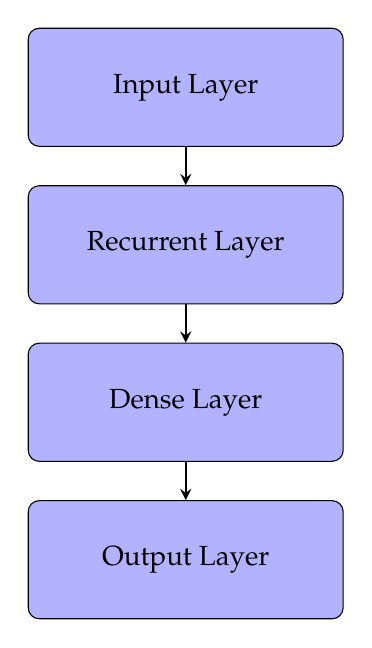
\begin{tikzpicture}[node distance=2cm]
		\node (i1) [startstop] {Input Layer};
		\node (i2) [startstop, below of=i1] {Recurrent Layer};
		
		\node (i3) [startstop, below of=i2] {Dense Layer};
		\node (i4) [startstop, below of=i3] {Output Layer};
		\draw [arrow] (i1) -- (i2) ;
		\draw [arrow] (i2) -- (i3);
		\draw [arrow] (i3) -- (i4);
		\end{tikzpicture}
	\end{center}
	\caption{Esquema de  RNN simple \\ Fuente:  \textit{Fuente Propia}}
\end{figure}


\subsection{LSTM simple}\label{LSTMESQUEMA}
\begin{figure}[H]
	\begin{center}
		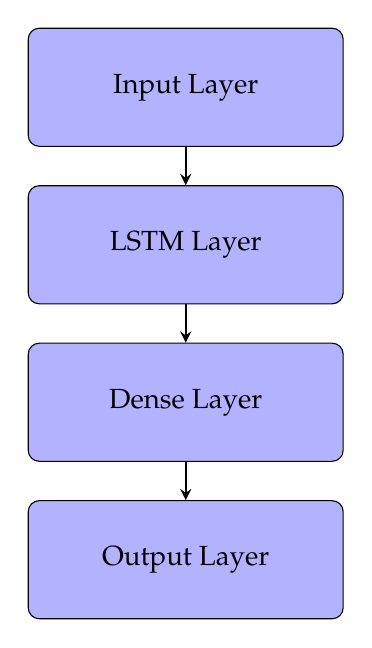
\begin{tikzpicture}[node distance=2cm]
		\node (i1) [startstop] {Input Layer};
		\node (i2) [startstop, below of=i1] {LSTM Layer};
		
		\node (i3) [startstop, below of=i2] {Dense Layer};
		\node (i4) [startstop, below of=i3] {Output Layer};
		\draw [arrow] (i1) -- (i2) ;
		\draw [arrow] (i2) -- (i3);
		\draw [arrow] (i3) -- (i4);
		\end{tikzpicture}
	\end{center}
	\caption{Esquema de LSTM simple \\ Fuente:  \textit{Fuente Propia}}
\end{figure}


\subsection{LSTM con Dropout}\label{LSTMESQUEMA1DROP}
\begin{figure}[H]
	\begin{center}
		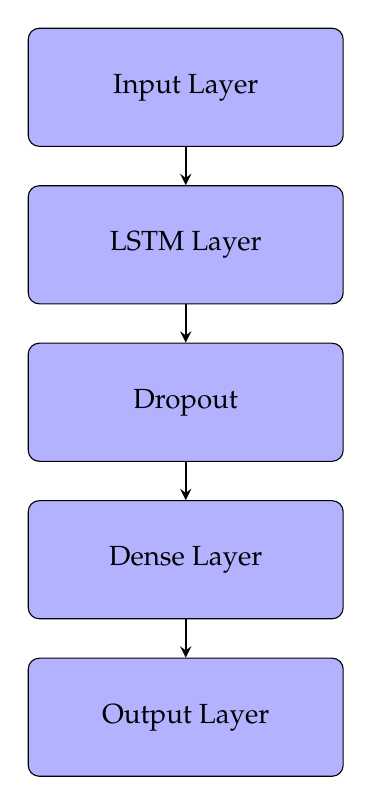
\begin{tikzpicture}[node distance=2cm]
		\node (i1) [startstop] {Input Layer};
		\node (i2) [startstop, below of=i1] {LSTM Layer};
		\node (i3) [startstop, below of=i2] {Dropout};
		\node (i4) [startstop, below of=i3] {Dense Layer};
		\node (i5) [startstop, below of=i4] {Output Layer};
		\draw [arrow] (i1) -- (i2) ;
		\draw [arrow] (i2) -- (i3);
		\draw [arrow] (i3) -- (i4);
		\draw [arrow] (i4) -- (i5);
		\end{tikzpicture}
	\end{center}
	\caption{Esquema de LSTM con dropout \\ Fuente:  \textit{Fuente Propia}}
\end{figure}

\subsection{2 capas LSTM  con 2 Dropout}\label{2LSTMESQUEMA}
\begin{figure}[H]
	\begin{center}
		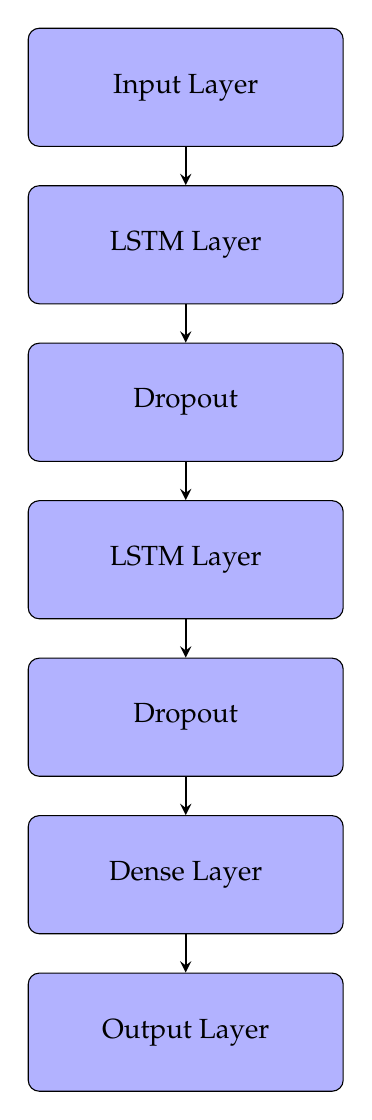
\begin{tikzpicture}[node distance=2cm]
		\node (i1) [startstop] {Input Layer};
		\node (i2) [startstop, below of=i1] {LSTM Layer};
		\node (i3) [startstop, below of=i2] {Dropout};
		\node (i4) [startstop, below of=i3] {LSTM Layer};
		\node (i5) [startstop, below of=i4] {Dropout};
		\node (i6) [startstop, below of=i5] {Dense Layer};
		\node (i7) [startstop, below of=i6] {Output Layer};
		\draw [arrow] (i1) -- (i2) ;
		\draw [arrow] (i2) -- (i3);
		\draw [arrow] (i3) -- (i4);
		\draw [arrow] (i4) -- (i5);
		\draw [arrow] (i5) -- (i6);
		\draw [arrow] (i6) -- (i7);
		\end{tikzpicture}
	\end{center}
	\caption{Esquema de 2 capas LSTM con 2 dropout \\ Fuente:  \textit{Fuente Propia}}
\end{figure}


\newpage
\section{Códigos}
\subsection{Conversión de formatos}\label{converter}
\begin{lstlisting}[language=Bash,caption=Bash para conversión de formato,captionpos=b]
# itera los archivos .ogg
for i in *.ogg;
# realiza la conversion ogg a wav usando ffmpeg
do ffmpeg -i "$i" "${i%.*}.wav"; 
done

\end{lstlisting}

\subsection{Obtención de coeficientes MFCC}\label{MFCCC}
\begin{lstlisting}[language=Python,caption=Obtención de MFCC,captionpos=b]
# cargado del audio
wave, sr = librosa.load(DIR+dir, mono=True)
# obtencion de los coeficientes
features= librosa.feature.mfcc(wave, sr,n_mfcc=20)
#padding con ceros asegurar misma dimension de salida
features=np.pad(features,((0,0),(0,160-len(features[0]))),
mode='constant',constant_values=0)

\end{lstlisting}

\subsection{One hot encoding}\label{onehot}

\begin{lstlisting}[language=Python,caption=one hot encoding,captionpos=b,xleftmargin=.05\textwidth]
from sklearn.preprocessing import OneHotEncoder
# vocabulario de clases definidas
vocabulary_words=np.array(['cero','uno','dos','tres',
'cuatro','cinco','seis','siete','ocho','nueve'])
onehot_encoder = OneHotEncoder(handle_unknown='ignore',
categories='auto')
# entrenamiento del OneHotEncoder
onehot_encoder.fit(X=vocabulary_words.reshape(-1,1))
\end{lstlisting}

\subsection{RNN}\label{RNNCODE}

\begin{lstlisting}[language=Python,caption=Modelo LSTM,captionpos=b,xleftmargin=.05\textwidth]
# establece la secuencia para empezar con el apilado de capas
model=tf.keras.Sequential()
# se apila una capa RNN simple 
model.add(tf.keras.layers.SimpleRNN(128, input_shape=(time_steps,n_inputs)))
# establece una capa densamente conectada
model.add(tf.layers.Dense(n_class, activation='softmax'))

\end{lstlisting}
\subsection{LSTM Simple}\label{LSTMCODE}
\begin{center}
	\begin{lstlisting}[language=Python,caption=Modelo LSTM,captionpos=b,xleftmargin=.05\textwidth]
	# usado para apilar las capas de la red
	model=tf.keras.Sequential()
	# apila una capa LSTM
	model.add(tf.keras.layers.LSTM(n_units,
	input_shape=(time_steps,n_inputs)))
	# establece una capa densamente conectada
	model.add(tf.layers.Dense(n_class, activation='softmax'))
	
	
	\end{lstlisting}
\end{center}
\subsection{LSTM con Dropout}\label{LSTMCODEDROP}

\begin{center}
	\begin{lstlisting}[language=Python,caption=Modelo LSTM,captionpos=b,xleftmargin=.05\textwidth]
	model=tf.keras.Sequential()
	# apila una capa LSTM
	model.add(tf.keras.layers.LSTM(n_units,
	input_shape=(time_steps,n_inputs)))
	# apila un Dropout a nuestra red para evitar overfitting
	model.add(tf.keras.layers.Dropout(0.5))
	# establece una capa densamente conectada
	model.add(tf.layers.Dense(n_class, activation='softmax'))
	
	
	\end{lstlisting}
\end{center}
\subsection{2 Capas LSTM con 2 Dropout}\label{2LSTM2DROPCODE}
\begin{center}
	\begin{lstlisting}[language=Python,caption=Modelo 2 capas LSTM y 2 dropout,captionpos=b,xleftmargin=.05\textwidth]
model=tf.keras.Sequential()
#primera capa LSTM
model.add(tf.keras.layers.LSTM(n_units, input_shape=(time_steps,n_inputs),return_sequences=True))
# aplicacion del Dropout
model.add(tf.keras.layers.Dropout(dropout))
# 2da capa LSTM
model.add(tf.keras.layers.LSTM(n_units, input_shape=(time_steps,n_inputs)))
# 2da aplicacion del Dropout
model.add(tf.keras.layers.Dropout(dropout))
model.add(tf.layers.Dense(n_class, activation='softmax'))
	\end{lstlisting}
\end{center}
\subsection{Configuración del modelo}\label{configmodel}
\begin{lstlisting}[language=Python,caption=Parámetros para el entrenamiento del modelo,captionpos=b,xleftmargin=.05\textwidth]
# configura el entrenamiento del modelo
model.compile(loss='categorical_crossentropy',
optimizer='adam',metrics=['accuracy'])
\end{lstlisting}
\subsection{Entrenamiento del modelo}\label{trainingmodel}
\begin{lstlisting}[language=Python,caption=Entrenamiento del modelo,captionpos=b,xleftmargin=.05\textwidth]
# entrenamiento del modelo pasando train and test set
history=model.fit(trainX,trainY,batch_size=batch_size,
epochs=n_epochs,validation_data=[testX,testY])
\end{lstlisting}

\section{Pruebas con RNN, LSTM con MFCC}
\subsection{Resultados de precisión de entrenamiento}\label{precision}
\subsubsection{64 estados ocultos}\label{64stateprec}
\begin{figure}[H]
	\centering
	\includegraphics[width=0.7\textwidth]{Figures/rnn_64_prec}
	\caption{Precisión de RNN para 64 estados ocultos\\ Fuente: {\textit{Fuente Propia}}}
	\label{RNNSIMPLE64}
\end{figure} 
\begin{figure}[H]
	\centering
	\includegraphics[width=0.7\linewidth]{Figures/lstm13_64_prec}
	\caption{Precisión de LSTM simple para 64 estados ocultos\\ Fuente: {\textit{Fuente Propia}}}
	\label{fig:lstm1364prec}
\end{figure}

\begin{figure}[H]
	\centering
	\includegraphics[width=0.7\linewidth]{Figures/lstm_64_05_prec}
	\caption{Precisión LSTM con dropout 0.5 para 64 estados ocultos\\ Fuente: {\textit{Fuente Propia}}}
	\label{fig:lstm6405prec}
\end{figure}
\begin{figure}[H]
	\centering
	\includegraphics[width=0.7\linewidth]{Figures/lstm_64_08_prec}
	\caption{Precisión LSTM con dropout 0.8 para 64 estados ocultos\\ Fuente: {\textit{Fuente Propia}}}
	\label{fig:lstm6408prec}
\end{figure}

\subsubsection{128 estados ocultos}\label{128stateprec}
\begin{figure}[H]
\centering
	\includegraphics[width=0.7\textwidth]{Figures/rnn_prec_400_13mfcc}
	\caption{Precisión de RNN para 128 estados ocultos\\ Fuente: {\textit{Fuente Propia}}}
	\label{RNNSIMPLE}
\end{figure} 

\begin{figure}[H]
	\centering
	\includegraphics[width=0.7\textwidth]{Figures/lstm_400_prec_13mfcc}
	\caption{Precisión de LSTM simple para 128 estados ocultos\\ Fuente: {\textit{Fuente Propia}}}
	\label{LSTMsimpel}
\end{figure} 

\begin{figure}[H]
	\centering
	\includegraphics[width=0.7\textwidth]{Figures/lstm_400drop05_prec_13mfcc}
	\caption{Precisión de LSTM dropout 0.5 para 128 estados ocultos\\ Fuente: {\textit{Fuente Propia}}}
	\label{LSTMdropout5}
\end{figure} 


\begin{figure}[H]
	\centering
	\includegraphics[width=0.7\textwidth]{Figures/lstm_400drop08_prec_13mfcc}
	\caption{Precisión de LSTM dropout 0.8 para 128 estados ocultos\\ Fuente: {\textit{Fuente Propia}}}
	\label{LSTMdropout8}
\end{figure} 
\newpage
\subsubsection{256 estados ocultos}\label{256stateprec}
\begin{figure}[H]
	\centering
	\includegraphics[width=0.7\linewidth]{Figures/rnn_256_prec}
	\caption{Precisión de RNN para 256 estados ocultos\\ Fuente: {\textit{Fuente Propia}}}
	\label{fig:rnn256prec}
	\centering
	\includegraphics[width=0.7\linewidth]{Figures/lstm_256_prec13}
	\caption{Precisión LSTM simple para 256 estados ocultos\\ Fuente: {\textit{Fuente Propia}}}
	\label{fig:lstm256prec13}
\end{figure}
\begin{figure}[H]
	\centering
	\includegraphics[width=0.7\linewidth]{Figures/lstm5_256_13prec}
	\caption{Precisión LSTM con dropout 0.5 para 256 estados ocultos\\ Fuente: {\textit{Fuente Propia}}}
	\label{fig:lstm525613prec}
	\centering
	\includegraphics[width=0.7\linewidth]{Figures/lst_256_13prec}
	\caption{Precisión LSTM con dropout 0.8 para 256 estados ocultos\\ Fuente: {\textit{Fuente Propia}}}
	\label{fig:lst25613prec}
\end{figure}
\newpage

\subsection{Resultados de función de perdida}

\subsubsection{64 Estados ocultos}\label{64statecost}
\begin{figure}[H]
	\centering
	\includegraphics[width=0.7\linewidth]{Figures/rnn_64_cost}
	\caption{Perdida LSTM para 64 estados ocultos\\ Fuente: {\textit{Fuente Propia}}}
	\label{fig:rnn64cost}

	\centering
	\includegraphics[width=0.7\linewidth]{Figures/lstm13_64_cost}
	\caption{Perdida LSTM  para 64 estados ocultos \\ Fuente: {\textit{Fuente Propia}}}
	\label{fig:lstm1364cost}
\end{figure}

\begin{figure}[H]
	\centering
	\includegraphics[width=0.7\linewidth]{Figures/lstm_64_05_cost}
	\caption{Perdida LSTM con dropout 0.5 para 64 estados ocultos\\ Fuente: {\textit{Fuente Propia}}}
	\label{fig:lstm6405cost}
	\centering
	\includegraphics[width=0.7\linewidth]{Figures/lstm_64_08_cost}
	\caption{Perdida LSTM con dropout 0.8 para 64 estados ocultos\\ Fuente: {\textit{Fuente Propia}}}
	\label{fig:lstm6408cost}
\end{figure}


\subsubsection{128 estados ocultos}\label{128statecost}
\begin{figure}[H]
	\centering
	\includegraphics[width=0.7\textwidth]{Figures/rnn_cost_400_13mfcc}
	\caption{Perdida de RNN para 128 estados ocultos\\ Fuente: {\textit{Fuente Propia}}}
	\label{RNNSIMPLEcost}
\end{figure} 


\begin{figure}[H]
	\centering
	\includegraphics[width=0.7\textwidth]{Figures/lstm_400_cost_13mfcc}
	\caption{Perdida de LSTM para 128 estados ocultos\\ Fuente: {\textit{Fuente Propia}}}
	\label{LSTMsimplecost}
\end{figure} 

\begin{figure}[H]
	\centering
	\includegraphics[width=0.7\textwidth]{Figures/lstm_400drop05_cost_13mfcc}
	\caption{Perdida de LSTM dropout 0.5 para 128 estados ocultos\\ Fuente: {\textit{Fuente Propia}}}
	\label{LSTMdropout5cost}
\end{figure} 


\begin{figure}[H]
	\centering
	\includegraphics[width=0.7\textwidth]{Figures/lstm_400drop08_cost_13mfcc}
	\caption{Perdida de LSTM dropout 0.8 para 128 estados ocultos\\ Fuente: {\textit{Fuente Propia}}}
	\label{LSTMdropout8cost}
\end{figure} 

\subsubsection{256 estados ocultos}\label{256statecost}
\begin{figure}[H]
	\centering
	\includegraphics[width=0.7\linewidth]{Figures/rnn_256_cost}
	\caption{Perdida de RNN para 256 estados ocultos\\ Fuente: {\textit{Fuente Propia}}}
	\label{fig:rnn256cost}

	\centering
	\includegraphics[width=0.7\linewidth]{Figures/lstm_256_cost13}
	\caption{Perdida de LSTM para 256 estados ocultos\\ Fuente: {\textit{Fuente Propia}}}
	\label{fig:lstm256cost13}
\end{figure}

\begin{figure}[H]
	\centering
	\includegraphics[width=0.7\linewidth]{Figures/lstm5_256_13cost}
	\caption{Perdida de LSTM con Dropout 0.5 para 256 estados ocultos\\ Fuente: {\textit{Fuente Propia}}}
	\label{fig:lstm525613cost}

	\centering
	\includegraphics[width=0.7\linewidth]{Figures/lstm_256_13cost}
	\caption{Perdida de LSTM con Dropout 0.8 para 256 estados ocultos\\ Fuente: {\textit{Fuente Propia}}}
	\label{fig:lstm25613cost}
\end{figure}

\newpage

\section{Propuesta de modelo para reconocimiento de voz}\label{modelo}

\subsection{Precisión}\label{precision_modelo}

\begin{figure}[H]
	\centering
	\includegraphics[width=0.7\linewidth]{Figures/MODEL_prec}
	\caption{Precisón de modelo con 2 LSTM y 2 Dropout 0.6}
	\label{fig:modelprec}
\end{figure}

\subsection{Error}\label{erro_modelo}

\begin{figure}[H]
	\centering
	\includegraphics[width=0.7\linewidth]{Figures/MODEL_cost}
	\caption{Error de modelo con 2 LSTM y 2 Dropout 0.6}
	\label{fig:modelcost}
\end{figure}

\end{document}